% -*- coding: utf-8; ispell-dictionary: "french"; -*-

%--------------
% Introduction
%--------------


Ce stage s'est déroulé au sein du projet $CERCLES^2$ \footnote{CERtification
Compositionnelle des Logiciels Embarqués critiqueS et Sûrs}, financé par l'Agence
Nationale de la Recherche. L'objectif du projet est de certifier formellement
des composants réutilisables, l'intérêt étant de réduire les tests en prouvant
grâce à des méthodes formelles la sûreté des différentes briques formant un
logiciel. L'intérêt est à la fois pratique par la réutilisabilité des composants
certifiés, et économique en réduisant le temps et le coût des tests. \\  

Un acteur majeur du développement de systèmes embarquées critiques est Scade,
un acronyme pour Safety Critical Application Developpement Environment. Cet
environnement de développement est basé sur la programmation graphique, par
schémas-blocs, permettant de définir des programmes faciles à lire et
permettant d'engendrer directement du code compilable (C ou ADA). Il est
notamment utilisé en aéronautique (grande partie du logiciel embarqué de
l'A380), dans le domaine spatial ou dans le nucléaire. Dans le cadre du projet,
c'est avec Scade que sont écrits les composants.\\

%% \begin{figure}[h]
%% \begin{center}
%% 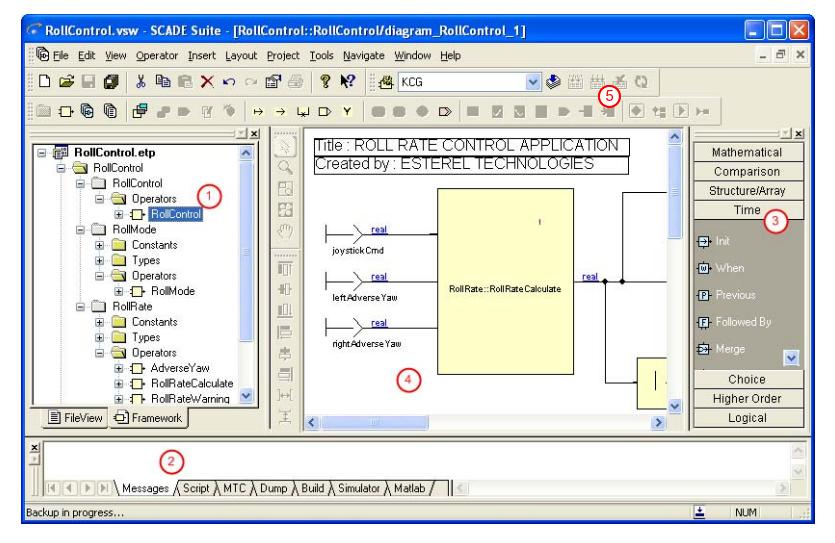
\includegraphics[scale=0.36]{intro_scade_pic.jpg}
%% \end{center}
%% \caption{Capture d'écran de l'envioronnement Scade}
%% \end{figure}

Pour assurer que ces composants sont sûrs et réutilisables, on
utilise une méthode formelle, qui permet d'exprimer la signification d'un
composant dans un formalisme mathématique, afin de démontrer leur
validité par rapport à une spécification.\\
Il faut alors introduire le concept des contrats: un contrat est
associé à un composant et impose des conditions sur ses entrées
(pré-conditions) et sur ses sorties (post-conditions). Ils formeront
ainsi une spécification du composant. Les contrats
ont été introduits par C.A.R Hoare, qui donne la définition
suivante: Soit $P$ et $R$ les pré-conditions et post-conditions associées au
programme $Q$, \\
%% \noindent
%% \fbox{
\begin{minipage}{\textwidth}
\begin{center}
$P\{Q\}R$ \\
\emph{"If the assertion P is true before initiation of a program Q, then the
assertion R will be true on its completion"}
\end{center}
\end{minipage}
%% }
\\
A partir d'un programme et de son contrat, il faut alors vérifier formellement
que: 
\begin{itemize}
\item  (i) Le programme est cohérent vis-à-vis de sa spécification.
\item (ii) l'initialisation du programme satisfait les pré-condition, et en
conséquence de (i) le résultat satisfait les post-conditions.
\end{itemize}
La validation est alors faite par une démonstration formelle.\\

Il existe différentes approches de démonstrations formelles, comme celle basée
sur des règles de typage des programmes, introduites par la correspondance de
Curry-Howard dans à la fin des années 50. 
L'avantage de la méthode choisie, la méthode B, est qu'elle a déjà
fait ses preuves industriellement, elle a notamment été utilisée pour
développer la ligne METEOR (ligne 14) du métro parisien, qui est
entièrement automatisée.\\ 
Elle a été introduite
par J.R. Abrial dans les années 80. Elle est basé sur le raffinement de
spécifications formelles vers une spécification exécutable. La spécification
formelle est rédigée dans un formalisme mathématique de haut niveau appelé
machine abstraite, dont le principe de calcul est basé sur le calcul
des prédicats du premier ordre étendu avec une théorie des
ensembles. Le raffinement de cette machine abstraite consiste à la
reformuler de façon plus concrète et à l'enrichir avec des
substitutions correspondants aux instructions du composant. Le
raffinement de plus bas niveau, exécutable, est appelé implantation. Il peut y
avoir des raffinements intermédiaires, mais nous n'aurons besoin que
d'une étape de raffinement de la machine abstraite vers l'implantation. Chaque
étape de raffinement passe par une étape d'obligations de preuves, une
validation par démonstration formelle, garantissant la fidélité de la
machine raffinée par rapport à la machine abrstraite. \\

Mon travail fut de développer un traducteur permettant de transposer un
composant écrit en SCADE vers B. Le traducteur suit une ligne de compilation classique, prenant en
entrée un code issu de Scade et produisant en sortie une machine abstraite
correspondant aux spécifications du contrat, ainsi que la machine raffinée qui
implante le programme. \\

\begin{figure}[h]
\begin{center}
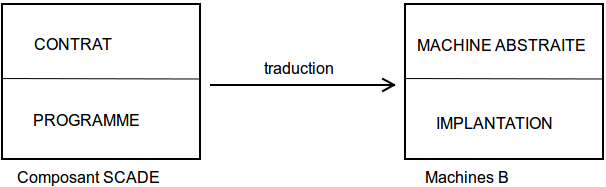
\includegraphics[scale=0.54]{intro_schema.png}
\end{center}
\caption{Schéma du principe de traduction}
\end{figure}
